%%%BEGIN+++++++++ induccionEM.tex +++++++++++++++++

El principio de inducción fue formulado por Michael Faraday  (Inglaterra) e independientemente por Joseph Henry (Estados Unidos) en el a\~no de 1831~\cite{}. Hoy en día, este principio es la base para producir la electricidad en la centrales hidroeléctricas que posteriormente es conducida hasta nuestros hogares.

\section{Flujo magnético}

\begin{figure}[h]
\begin{center}
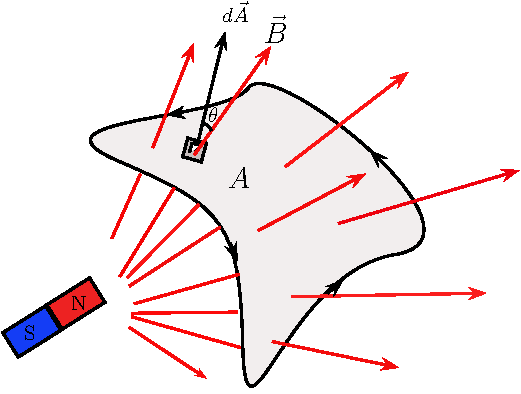
\includegraphics[scale=0.8]{induccionEM/flujoB-definicion.pdf}
\end{center}
\caption{Flujo magnético atravezando la superficie $A$.}
\label{fig:flujoB-def}
\end{figure}
%
Se define el flujo agnético $\Phi_B$ a través de la superficie de área $A$ como
\begin{align}
\Phi_B=\int_A \vec{B}\cdot d\vec{A}\,,
\end{align}
donde $d\vec{A}$ es un vector normal a la superficie, y forma un ángulo $\theta$ con el vector $\vec{B}$, tal como se muesstra en la Fig.~\ref{fig:flujoB-def}. La integral debe realizarse sobre toda el área $A$. 

\section{Principio de inducción}

%%%END+++++++++ induccionEM ++++++++++++++++++++++